Chúng ta ước tính rằng dân số thế giới vào năm 1993 là
\[
P(43) = 2560e^{0{,}017185(43)} \approx 5360\text{ triệu}
\]
Mô hình dự đoán rằng dân số vào năm 2025 sẽ là
\[
P(75) = 2560e^{0{,}017185(75)} \approx 9289\text{ triệu}
\]
Đồ thị trong Hình 1 cho thấy mô hình khá chính xác cho đến cuối thế kỷ 20 (các điểm biểu diễn dân số thực tế), vì vậy ước tính cho năm 1993 là khá đáng tin cậy. Nhưng dự đoán cho năm 2025 có thể không chính xác như vậy.

\vspace{0.8em}
\noindent\makebox[0pt][r]{%
  \begin{minipage}[b]{36mm}
    \raggedright
    \textbf{\textsf{HÌNH 1}}\\[3pt]
    {\small Mô hình cho sự tăng trưởng dân số thế giới trong nửa sau thế kỷ 20}
  \end{minipage}\hspace{6mm}%
}%
\begin{minipage}[b]{\linewidth}
  \hspace*{12mm}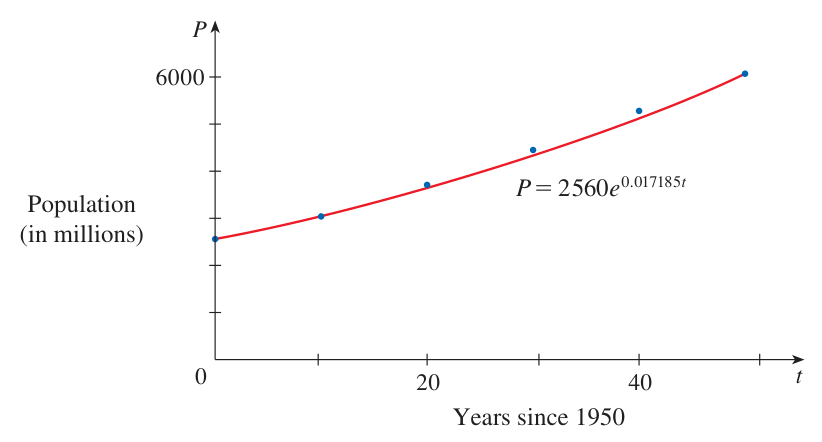
\includegraphics[width=0.76\linewidth]{images/p0276_fig1.png}%
  \hfill\raisebox{2pt}{\color{stewartcyan}\rule{1.1ex}{1.1ex}}
\end{minipage}

\vspace{1.2em}
\noindent{\color{stewartcyan}\rule{1.1ex}{1.1ex}}\hspace{0.5em}\textbf{\textsf{\large Phân rã phóng xạ}}\par\vspace{0.3em}
Các chất phóng xạ phân rã bằng cách tự phát ra bức xạ. Nếu $m(t)$ là khối lượng còn lại từ khối lượng ban đầu $m_0$ của chất sau thời gian $t$, thì tốc độ phân rã tương đối
\[
-\frac{dm/dt}{m}
\]
được tìm thấy bằng thực nghiệm là một hằng số. (Vì $dm/dt$ âm nên tốc độ phân rã tương đối là dương.) Từ đó suy ra
\[
\frac{dm}{dt} = km
\]
trong đó $k$ là một hằng số âm. Nói cách khác, các chất phóng xạ phân rã với tốc độ tỉ lệ thuận với khối lượng còn lại. Điều này có nghĩa là chúng ta có thể sử dụng Định lý 2 để chỉ ra rằng khối lượng phân rã theo hàm mũ:
\[
m(t) = m_0 e^{kt}
\]
Các nhà vật lý biểu diễn tốc độ phân rã theo \textbf{chu kỳ bán rã}, thời gian cần thiết để một nửa của một lượng chất bất kỳ phân rã.

\vspace{1.0em}
\noindent\textbf{\textsf{\color{stewartcyan}VÍ DỤ 2}}\hspace{0.8em}Chu kỳ bán rã của radium-226 là 1590 năm.
\begin{enumerate}[label=\textsf{\textbf{(\alph*)}}, leftmargin=2em, itemsep=1.5pt, parsep=0pt, topsep=2pt]
  \item Một mẫu radium-226 có khối lượng $100\text{ mg}$. Hãy tìm công thức tính khối lượng của mẫu còn lại sau $t$ năm.
  \item Tìm khối lượng còn lại sau 1000 năm làm tròn đến miligam gần nhất.
  \item Khi nào khối lượng sẽ giảm xuống còn $30\text{ mg}$?
\end{enumerate}

\vspace{0.6em}
\noindent\textbf{\textsf{\color{stewartcyan}LỜI GIẢI}}
\begin{enumerate}[label=\textsf{\textbf{(\alph*)}}, leftmargin=2em, itemsep=1.5pt, parsep=0pt, topsep=2pt]
  \item Gọi $m(t)$ là khối lượng của radium-226 (tính bằng miligam) còn lại sau $t$ năm. Khi đó $dm/dt = km$ và $m(0) = 100$, do đó Định lý 2 cho ta
  \[
  m(t) = m(0)e^{kt} = 100e^{kt}
  \]
\end{enumerate}
